\chapter{Experiments}
\begin{itemize}
    \item Was wird getestet?
\end{itemize}
\section{Experimental Design}
\begin{figure}[H]
\centering


\tikzset{every picture/.style={line width=0.75pt}} %set default line width to 0.75pt        

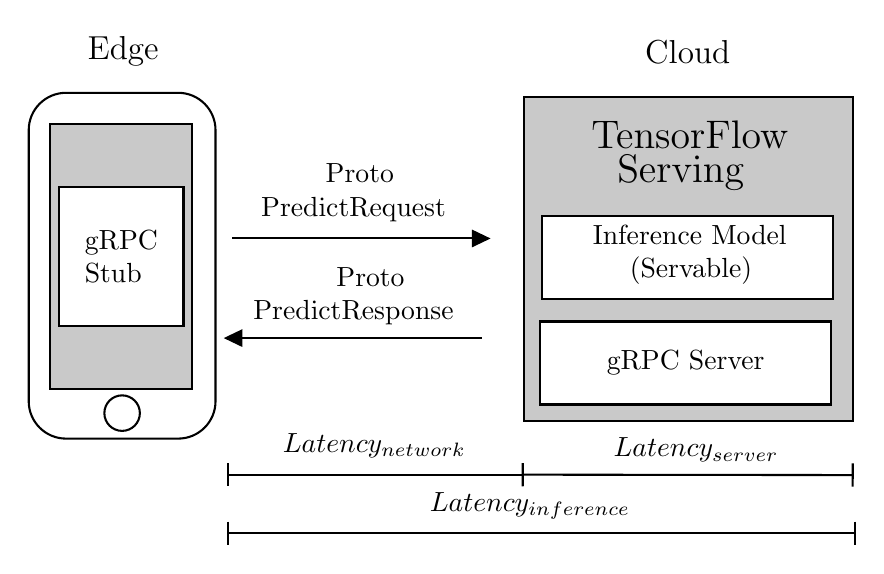
\begin{tikzpicture}[x=0.75pt,y=0.75pt,yscale=-1,xscale=1]
%uncomment if require: \path (0,300); %set diagram left start at 0, and has height of 300

%Straight Lines [id:da7072764839644827] 
\draw    (149.5,291) -- (451.5,291) ;
\draw [shift={(451.5,291)}, rotate = 180] [color={rgb, 255:red, 0; green, 0; blue, 0 }  ][line width=0.75]    (0,5.59) -- (0,-5.59)   ;
\draw [shift={(149.5,291)}, rotate = 180] [color={rgb, 255:red, 0; green, 0; blue, 0 }  ][line width=0.75]    (0,5.59) -- (0,-5.59)   ;
%Straight Lines [id:da9536138531960994] 
\draw    (291.5,262.8) -- (450.5,263) ;
\draw [shift={(450.5,263)}, rotate = 180.07] [color={rgb, 255:red, 0; green, 0; blue, 0 }  ][line width=0.75]    (0,5.59) -- (0,-5.59)   ;
\draw [shift={(291.5,262.8)}, rotate = 180.07] [color={rgb, 255:red, 0; green, 0; blue, 0 }  ][line width=0.75]    (0,5.59) -- (0,-5.59)   ;
%Shape: Rectangle [id:dp8902536871651789] 
\draw  [fill={rgb, 255:red, 201; green, 201; blue, 201 }  ,fill opacity=1 ] (63.91,93.69) -- (132.34,93.69) -- (132.34,221.63) -- (63.91,221.63) -- cycle ;
%Rounded Rect [id:dp41557214204551274] 
\draw   (53.5,96.82) .. controls (53.5,86.88) and (61.56,78.82) .. (71.5,78.82) -- (125.5,78.82) .. controls (135.44,78.82) and (143.5,86.88) .. (143.5,96.82) -- (143.5,227.43) .. controls (143.5,237.37) and (135.44,245.43) .. (125.5,245.43) -- (71.5,245.43) .. controls (61.56,245.43) and (53.5,237.37) .. (53.5,227.43) -- cycle ;
%Shape: Ellipse [id:dp8878397246816687] 
\draw   (89.95,233.16) .. controls (89.95,228.43) and (93.78,224.6) .. (98.5,224.6) .. controls (103.22,224.6) and (107.05,228.43) .. (107.05,233.16) .. controls (107.05,237.88) and (103.22,241.71) .. (98.5,241.71) .. controls (93.78,241.71) and (89.95,237.88) .. (89.95,233.16) -- cycle ;
%Straight Lines [id:da5813802620369573] 
\draw    (151.48,149) -- (274,149) ;
\draw [shift={(276,149)}, rotate = 540] [fill={rgb, 255:red, 0; green, 0; blue, 0 }  ][line width=0.75]  [draw opacity=0] (8.93,-4.29) -- (0,0) -- (8.93,4.29) -- cycle    ;

%Straight Lines [id:da16220168680973557] 
\draw    (149.48,197) -- (272,197) ;

\draw [shift={(147.48,197)}, rotate = 360] [fill={rgb, 255:red, 0; green, 0; blue, 0 }  ][line width=0.75]  [draw opacity=0] (8.93,-4.29) -- (0,0) -- (8.93,4.29) -- cycle    ;
%Shape: Rectangle [id:dp8411150472244695] 
\draw  [fill={rgb, 255:red, 201; green, 201; blue, 201 }  ,fill opacity=1 ] (292,81) -- (450.5,81) -- (450.5,237) -- (292,237) -- cycle ;
%Shape: Rectangle [id:dp13557861576626729] 
\draw  [fill={rgb, 255:red, 255; green, 255; blue, 255 }  ,fill opacity=1 ] (301,138) -- (441,138) -- (441,178) -- (301,178) -- cycle ;
%Shape: Rectangle [id:dp5681963435258506] 
\draw  [fill={rgb, 255:red, 255; green, 255; blue, 255 }  ,fill opacity=1 ] (68.19,124.22) -- (128.07,124.22) -- (128.07,191.1) -- (68.19,191.1) -- cycle ;
%Shape: Rectangle [id:dp7458124222136935] 
\draw  [fill={rgb, 255:red, 255; green, 255; blue, 255 }  ,fill opacity=1 ] (300,189) -- (440,189) -- (440,229) -- (300,229) -- cycle ;
%Straight Lines [id:da6846625455377753] 
\draw    (149.5,262.8) -- (291.5,262.8) ;
\draw [shift={(291.5,262.8)}, rotate = 180] [color={rgb, 255:red, 0; green, 0; blue, 0 }  ][line width=0.75]    (0,5.59) -- (0,-5.59)   ;
\draw [shift={(149.5,262.8)}, rotate = 180] [color={rgb, 255:red, 0; green, 0; blue, 0 }  ][line width=0.75]    (0,5.59) -- (0,-5.59)   ;

% Text Node
\draw (375,251) node  [align=left] {$\displaystyle Latency_{server}$$ $};
% Text Node
\draw (210,127) node  [align=left] { \ \ \ \ \ \ \ Proto\\PredictRequest};
% Text Node
\draw (99,59) node  [align=left] {{\large Edge}};
% Text Node
\draw (371,59) node  [align=left] {{\large Cloud}};
% Text Node
\draw (372,109) node  [align=left] {{\Large TensorFlow}\\{\Large  \ \ Serving}};
% Text Node
\draw (372,157) node  [align=left] {Inference Model\\ \ \ \ \ (Servable)};
% Text Node
\draw (210,177) node  [align=left] { \ \ \ \ \ \ \ \ \ Proto\\PredictResponse};
% Text Node
\draw (98.13,157.66) node  [align=left] {gRPC\\ Stub};
% Text Node
\draw (370,209) node  [align=left] {gRPC Server};
% Text Node
\draw (220,249) node  [align=left] {$\displaystyle Latency_{network}$$ $};
% Text Node
\draw (295,278) node  [align=left] {$\displaystyle Latency_{inference}$$ $};


\end{tikzpicture}
\caption{placeholder}
\label{fig:cloud}
\end{figure}
\begin{figure}[H]
\centering



\tikzset{every picture/.style={line width=0.75pt}} %set default line width to 0.75pt        

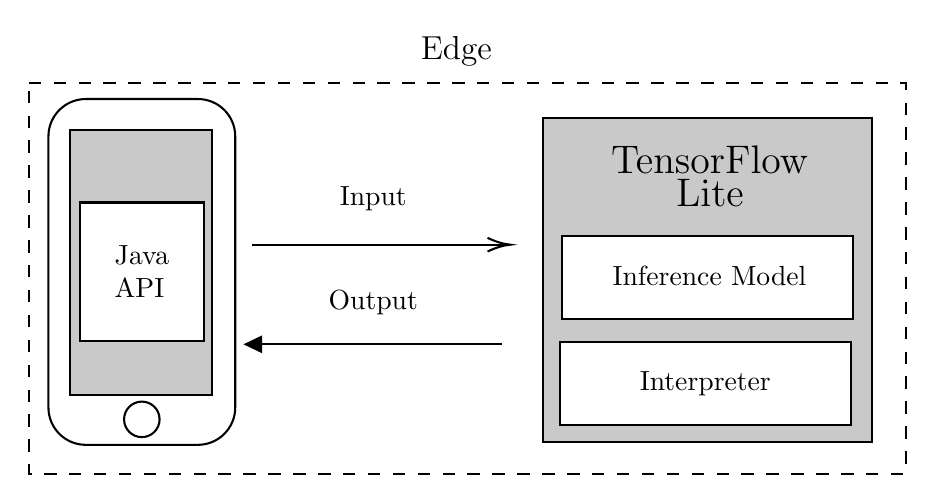
\begin{tikzpicture}[x=0.75pt,y=0.75pt,yscale=-1,xscale=1]
%uncomment if require: \path (0,300); %set diagram left start at 0, and has height of 300

%Shape: Rectangle [id:dp13292222689234756] 
\draw  [fill={rgb, 255:red, 201; green, 201; blue, 201 }  ,fill opacity=1 ] (61.91,111.69) -- (130.34,111.69) -- (130.34,239.63) -- (61.91,239.63) -- cycle ;
%Rounded Rect [id:dp7897713915001106] 
\draw   (51.5,114.82) .. controls (51.5,104.88) and (59.56,96.82) .. (69.5,96.82) -- (123.5,96.82) .. controls (133.44,96.82) and (141.5,104.88) .. (141.5,114.82) -- (141.5,245.43) .. controls (141.5,255.37) and (133.44,263.43) .. (123.5,263.43) -- (69.5,263.43) .. controls (59.56,263.43) and (51.5,255.37) .. (51.5,245.43) -- cycle ;
%Shape: Ellipse [id:dp9670901006981827] 
\draw   (87.95,251.16) .. controls (87.95,246.43) and (91.78,242.6) .. (96.5,242.6) .. controls (101.22,242.6) and (105.05,246.43) .. (105.05,251.16) .. controls (105.05,255.88) and (101.22,259.71) .. (96.5,259.71) .. controls (91.78,259.71) and (87.95,255.88) .. (87.95,251.16) -- cycle ;
%Straight Lines [id:da9993479608904674] 
\draw    (149.48,167) -- (272,167) ;
\draw [shift={(274,167)}, rotate = 540] [color={rgb, 255:red, 0; green, 0; blue, 0 }  ][line width=0.75]    (10.93,-3.29) .. controls (6.95,-1.4) and (3.31,-0.3) .. (0,0) .. controls (3.31,0.3) and (6.95,1.4) .. (10.93,3.29)   ;

%Straight Lines [id:da5401559459790608] 
\draw    (147.48,215) -- (270,215) ;

\draw [shift={(145.48,215)}, rotate = 360] [fill={rgb, 255:red, 0; green, 0; blue, 0 }  ][line width=0.75]  [draw opacity=0] (8.93,-4.29) -- (0,0) -- (8.93,4.29) -- cycle    ;
%Shape: Rectangle [id:dp45054130026891115] 
\draw  [fill={rgb, 255:red, 201; green, 201; blue, 201 }  ,fill opacity=1 ] (290,106) -- (448.5,106) -- (448.5,262) -- (290,262) -- cycle ;
%Shape: Rectangle [id:dp21016153851852382] 
\draw  [fill={rgb, 255:red, 255; green, 255; blue, 255 }  ,fill opacity=1 ] (299,163) -- (439,163) -- (439,203) -- (299,203) -- cycle ;
%Shape: Rectangle [id:dp8946256165796296] 
\draw  [fill={rgb, 255:red, 255; green, 255; blue, 255 }  ,fill opacity=1 ] (298,214) -- (438,214) -- (438,254) -- (298,254) -- cycle ;
%Shape: Rectangle [id:dp1345031923489386] 
\draw  [dash pattern={on 4.5pt off 4.5pt}] (42,89) -- (464.5,89) -- (464.5,277.4) -- (42,277.4) -- cycle ;
%Shape: Rectangle [id:dp7242946292477495] 
\draw  [fill={rgb, 255:red, 255; green, 255; blue, 255 }  ,fill opacity=1 ] (66.56,146.69) -- (126.44,146.69) -- (126.44,213.56) -- (66.56,213.56) -- cycle ;

% Text Node
\draw (208,145) node  [align=left] {Input};
% Text Node
\draw (248,74) node  [align=left] {{\large Edge}};
% Text Node
\draw (370,134) node  [align=left] {{\Large TensorFlow}\\{\Large  \ \ \ \ \ Lite}};
% Text Node
\draw (370,182) node  [align=left] {Inference Model};
% Text Node
\draw (208,195) node  [align=left] {Output};
% Text Node
\draw (368,234) node  [align=left] {Interpreter};
% Text Node
\draw (96.5,180.12) node  [align=left] {Java\\ API};


\end{tikzpicture}
\caption{placeholder}
\label{fig:edge}
\end{figure}
\subsection{Hardware}
\subsubsection{Edge}
Pixel 3
\subsubsection{Cloud}
DGX-1
\subsection{Frameworks}
\begin{itemize}
    \item Tensorflow Serrving
    \item Tensorflow Lite
\end{itemize}
\subsection{Models}
\begin{itemize}
    \item MobileNet
    \item ResNet
\end{itemize}

\section{Instantiation}
\begin{itemize}
    \item Wie wurde was gtestestet?
\end{itemize}
\section{Evaluation}
\begin{itemize}
    \item Haufen Graphen
    \item Was kann man aus Graphen schließen?
    \item Handlungsempfehlung
\end{itemize}
\endinput 
